\chapter{BACKGROUND} \label{chap:background}
In this section, we provide the background necessary for understanding the design of iGen. In Section~\ref{ti}, we describe Threat intelligence and how it is consumed by security tools. Then, in Section~\ref{cnn}, we describe Convolutional Neural Network (CNN) and how it can be used in iGen.  

\section{Threat Intelligence} \label{ti}

Given the increasing number and rapidly evolving nature of current threats, quick sharing and exchange of relevant threat information is the key to swiftly detecting, understanding, and responding to cyber-attacks. Threat intelligence is two things: (1) a process of collection of knowledge that defines security threats, which empowers an organization to determine its responses at the strategic, operational, and tactical levels, and (2) information that has been analyzed to discover actionable insights. Actionable threat intelligence is insight that an organization can act on—--it enables informed decision-making that results in improved outcomes. 

Threat intelligence consists of two words: ``Threat'' and ``Intelligence''. ``Threat'' is an agent (that is, a menace or hazard) that takes advantage of the vulnerability. Whereas, ``Intelligence'' can be defined as: 
\begin{itemize}
 \item[$\bullet$ ] Act of generating new information by correlating information from different sources.
  \item[$\bullet$ ] Capacity to know or understand.
  \item[$\bullet$ ] Knowledge imparted through study, research or experience.
\end{itemize}


\subsection{Consumption of Threat Intelligence}

Indicators of Compromise (IOCs) are used for organizations to exchange threat intelligence. There are different standards for IOCs which includes OpenIOC, STIX, and snort rules. OpenIOC was introduced by Mandiant in 2011.  It is primarily used in Mandiant products, but has also been released as an open standard. OpenIOC provides definitions for specific technical details including over 500 indicator terms. Adding new terms is easy because the terms are separated from the main schema. Most of the terms are host-centric.

Similarly, STIX is another format for storing IOCs. STIX allows defining threat information, including threat details, as well as the \emph{context} of the threat. STIX is developed by Mitre, and is designed to support four cyber threat use cases: investigating cyber threats, stating indicator patterns, response activities management, and sharing threat information. STIX uses XML to define threat-related constructs such as exploit target, campaign, indicator, threat actor, and TTP.

Snort is an open-source network intrusion prevention system (IPS)~\cite{sekar}, which  executes real-time traffic analysis and packet-logging on IP networks. It is also capable of performing protocol analysis, content searching, and matching, and can be used to detect a variety of attacks and probes, such as buffer overflows, stealth port scans, CGI attacks, SMB probes, OS fingerprinting attempts, and more. Snort uses a rule language to describe traffic that it should collect or pass, as well as a detection engine that uses a modular plug-in architecture. Rules created using this language are called snort rules.

Suricata rules are the defacto method for sharing and matching threat intelligence against network traffic. A suricata rule has three components: The action, header and rule-options.
%Adam: The above paragraph needs more information

%iGen has capabilities to transform IOCs related to particular event or incident into different output formats mentioned above.  These output formats can be directly consumed by different security mechanisms like IDS, IPS etc. This helps iGen further reduce the manual task of converting the IOCs into different rules/formats. 

\section{Convolutional Neural Network Architecture} \label{cnn}

Recently, different models based on deep learning have achieved significant results in computer vision and speech recognition. Convolutional Neural Networks (CNNs) were responsible for major breakthroughs in image classification~\cite{krizhevsky} and are the core of most computer vision systems today, from Facebook's automated photo tagging~\cite{stone} to self-driving cars~\cite{bojarski}. 

In the case of Natural Language Processing (NLP), much of the work that uses deep learning methods involves learning word vector representations through neural language models and performing composition over the learned word vectors for classification tasks. Word vectors, wherein words are projected from a sparse, 1-of-$V$ encoding (here $V$ is the vocabulary size) onto a lower dimensional vector space via a hidden layer, are essentially feature extractors that encode semantic features of words in their dimensions. In such compact representations, semantically close words are likewise close--in euclidean or cosine distance---in the lower dimensional vector space~\cite{mikolov}.

Recently, researchers have also started applying CNNs with word embeddings to problems in Natural Language Processing (NLP) and got some interesting results. CNNs utilize layers with convolving filters that are applied to local features. CNNs are effective for NLP and have achieved excellent results in semantic parsing, search query retrieval, sentence modeling, and other traditional NLP tasks.

\subsection{Convolution}
%
%\begin{figure}
%  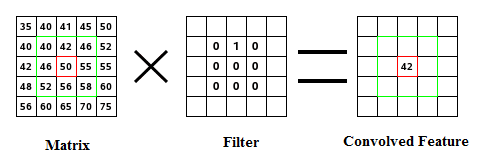
\includegraphics[width=\linewidth]{convolution.jpg}
%  \caption{Convolution with 3x3 filter.}
%  \label{fig:lifecycle}
%\end{figure}

%Convolution is a sliding window function applied to a matrix. As shown in figure 2, matrix on the left represents a black and white image. Each entry in the matrix corresponds to one pixel, 0 for black and 1 for white. The sliding window is called a kernel, filter, or feature detector. Here we use a $3\times3$ filter, multiply its values element-wise with the original matrix, then sum them up. To get the full convolution we do this for each element by sliding the filter over the whole matrix. Final matrix created after applying the filter is called convolved feature. 

Convolution~\cite{hu} is a sliding window function applied to a matrix. The sliding window is called a kernel, filter, or feature detector. Here we use a $N\times N$ filter, multiply its values element-wise with the original matrix, then sum them. To get the full convolution we do this for each element by sliding the filter over the whole matrix. Final matrix created after applying the filter is called convolved feature. 


\subsection{Convolution Neural Network}
CNNs are fundamentally several layers of convolutions with nonlinear activation functions like rectified linear unit (ReLU)~\cite{nair} or hyperbolic tangent (tanh)~\cite{goodfellow} applied to the results. In a traditional feedforward neural network, each input neuron to each output neuron in the next layer. It is called as fully connected layer, or affine layer. But it's different in case of CNNs. CNNs use convolutions over the input layer to compute the output. This results in local connections, where each region of the input is connected to a neuron in the output. Each convolution layer applies different filters, characteristically hundreds or thousands, and combines their results. Then pooling is performed using the pooling (subsampling) layer. We will discuss more in Chapter 4. CNN automatically learns the values of its filters based on the task during the training phase. For example, in image classification a CNN learns to detect edges from raw pixels in the first layer, then uses the edges to detect simple shapes in the second layer, and then uses these shapes to deter higher-level features, such as facial shapes in higher layers. The last layer is then a classifier that uses these high-level features. 



In the case of iGen, input to a CNN is sentences extracted from blog articles and security reports instead of image pixels. Each sentence is represented as a matrix. Each row vector of the matrix corresponds to one token, typically a word. That is, each row is vector that represents a word. These vectors might be, e.g., outputs from trained word2vec or GloVe~\cite{pennington} models. We will discuss more about the iGen CNN in Section 3.2. 



%CNNs are fundamentally several layers of convolutions with nonlinear activation functions like rectified linear unit (ReLU) or hyperbolic tangent (tanh) applied to the results. In a traditional feedforward neural network, each input neuron to each output neuron in the next layer. It is called as fully connected layer, or affine layer. But it’s different in case of CNNs. CNNs use convolutions over the input layer to compute the output. This results in local connections, where each region of the input is connected to a neuron in the output. Each convolution layer applies different filters, characteristically hundreds or thousands like the ones showed above in figure 2, and combines their results. Then pooling is performed using the pooling (subsampling) layer, we will talk more about it in section 3. CNN automatically learns the values of its filters based on the task during the training phase. For example, in Image Classification a CNN learn to detect edges from raw pixels in the first layer, then use the edges to detect simple shapes in the second layer, and then use these shapes to deter higher-level features, such as facial shapes in higher layers. The last layer is then a classifier that uses these high-level features. . A simple CNN is shown in the figure 3. 
%
%
%\begin{figure}
%  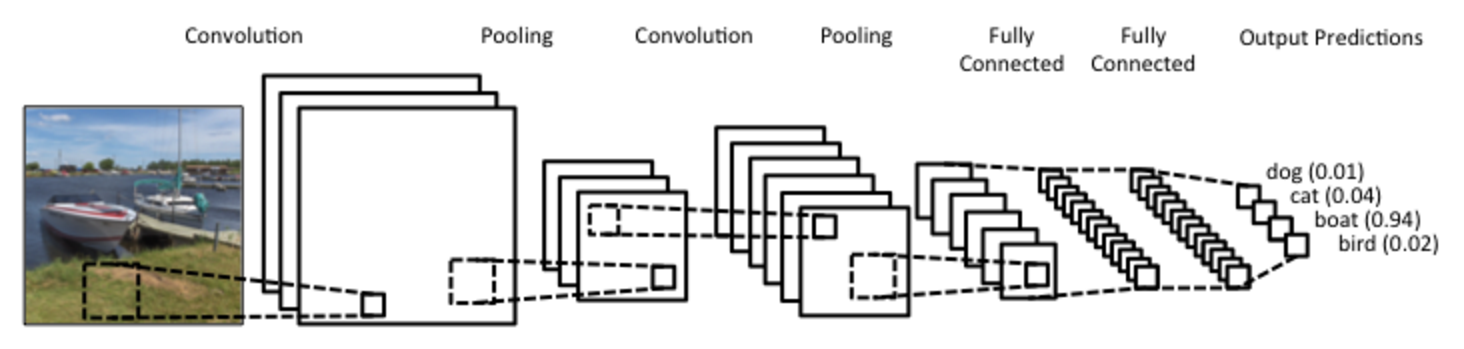
\includegraphics[width=\linewidth]{CNN.jpg}
%  \caption{Convolutional Neural Network (CNN) applied on an image.}
%  \label{fig:cnn}
%\end{figure}
%
%In case of iGen, input to CNN is sentences extracted from blog articles and security reports instead of image pixels. Each sentence is represented as a matrix. Each row vector of the matrix corresponds to one token, typically a word. That is, each row is vector that represents a word. These vectors might be, e.g., outputs from trained word2vec [] or GloVe [] models. We denote the dimensionality of the word vectors by $d$. If the length of a given sentence is $l$, then the dimensionality of the sentence matrix is $l \times d$. Here, sentences matrix can be effectively treated as an ‘image’, and perform convolution on it via linear filters. In text applications there is inherent sequential structure to the data. Because rows represent discrete symbols (namely, words), it is reasonable to use filters with widths equal to the dimensionality of the word vectors (i.e., $d$). Hence we can merely vary the ‘height’ of the filter, i.e., the number of adjacent rows considered jointly. We will refer to the height of the filter as the \emph{region size} of the filter [Collobert and Weston (2008)].
%
%Assume that a filter represented by the weight matrix $\mathbf{w}$ with region size $h$; $\mathbf{w}$ will contain $h \cdot d$ parameters to be estimated. Sentence matrix can be denoted by $\mathbf{S}\in \mathbb{R}^{l\times d}$ , and $\mathbf{S}[i:j]$ is used to represent the sub-matrix of  $\mathbf{S}$ from row $i$ to row $j$. The output sequence $\mathbf{out}\in\mathbb{R}^{l-h+1}$ of the convolution operator is obtained by repeatedly applying the filter on sub-matrices of $\mathbf{S}$:
%
%\begin{equation}
%out_i = \mathbf{w}\cdot \mathbf{S}[i:i+h-1], 
%\end{equation}
%
%\noindent where $i=1 \ldots l-h+1$, and $\cdot$ is the dot product(or sum over element-wise multiplications) between the sub-matrix and the filter. A bias term is added $c\in \mathbb{R}$ and an activation function (ReLU or tanh) $f$ is applied to each $out_i$, inducing the \emph{feature map} $\mathbf{fout} \in \mathbb{R}^{l-h+1}$ for this filter:
%
%\begin{equation}
%fout_i = f(out_i+c).
%\end{equation}
%
%\noindent Multiple filters are used for the same region size to learn complementary features from the same regions. Alternately, multiple kinds of filters with different region sizes (i.e., `heights') can be used.
%
%The dimensionality of the feature map created by each filter depends on the sentence length and the filter region size (i.e., $h$). On each feature map, a pooling function is applied to induce a fixed-length vector. A common strategy is \emph{1-max pooling} ~\cite{boureau2010theoretical}, which selects the largest number from each feature map. 
%
%All outputs generated from each filter map after 1-max pooling can be concatenated into a fixed-length, `top-level' feature vector. This vector is then fed through a softmax function to generate the final classification. At this softmax layer, `dropout'~\cite{hinton2012improving} is applied as a means of regularization in order to prevent model from overfitting. This involves randomly setting values in the weight vector to 0. One may also impose an $l2$ norm constraint, i.e., linearly scale the $l2$ norm of the vector to a pre-specified threshold when it exceeds this. Fig.~\ref{fig:CNNarc} provides a schematic illustrating the model architecture just described. 
%
%Objective during training to minimize the categorical cross-entropy loss. The parameters to be estimated include the weight vector(s) of the filter(s), the bias term in the activation function, and the weight vector of the softmax function. In our approach which is ‘non-static’, we also tuned the word vectors. Optimization is performed using Stochastic Gradient Descent (SGD) and back-propagation~\cite{rumelhart1988learning}.